\section{4-bit Carry Look-ahead Adder(CLA)}
\text{The Carry Look-ahead adder eliminates the need to wait for the carry from the preceding block to ripple when using a ripple carry adder, reducing the time it takes to calculate the sum of two values. The carry look-ahead adder's logic and circuit schematic are as follows:-}
\subsection{Circuit Diagram}
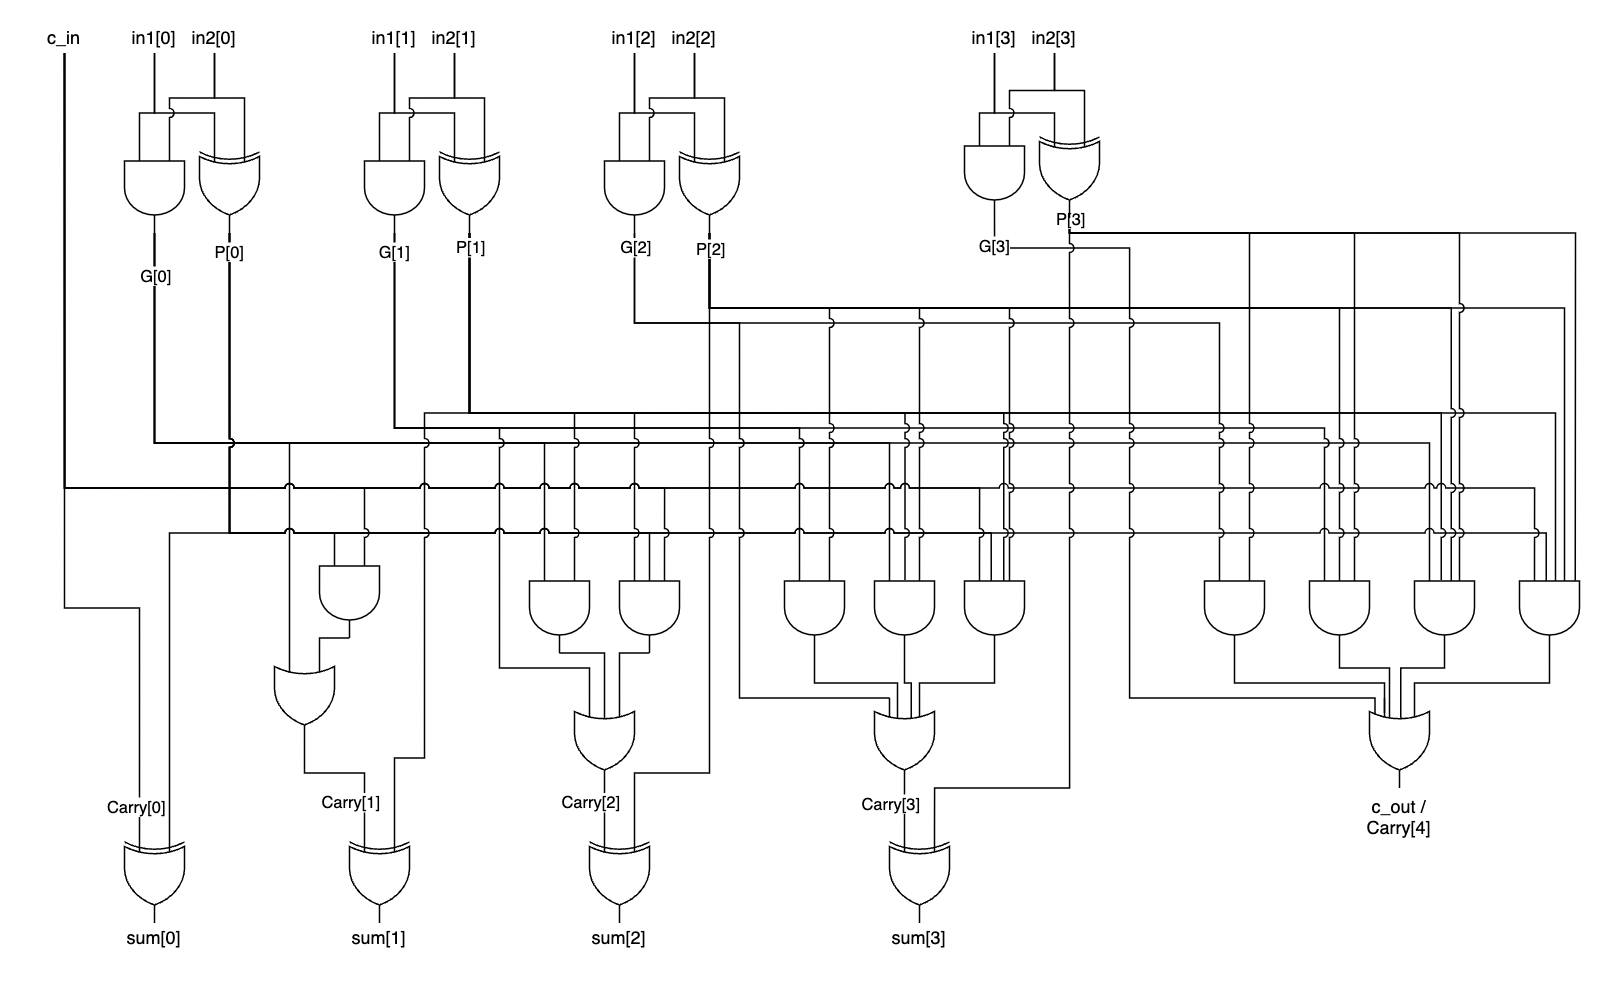
\includegraphics[width = 18cm]{images/cla_4_bit.png}
\subsection{Logic Expression}
Logic of the Circuit:-
$$ P =  a \oplus b $$ 
$$ G =  a \And b $$
Expanding for i,
\begin{equation} P[i] = a[i] \oplus b[i] \hspace{0.05in} \textbf{for all 0<=i<=3} \end{equation}
\begin{equation} G[i] = a[i] \And b[i] \hspace{0.05in} \textbf{for all 0<=i<=3} \end{equation}
Initialize C[0] to be $c_{in}$
Then Recursively we can elaborate:-
\begin{equation} s[i] = P[i] \oplus C[i] \hspace{0.08 in} \text{0<=i<=3} \begin{equation}
\begin{equation}C[i] = G[i-1]  |  (P[i-1] \and C[i-1]) \hspace{0.07 in} \text{for all 1<=i<=4}\end{equation}\\

\begin{equation}C0 = c_{in} \begin{equation} \\
\begin{equation}C1 = G[0] | (P[0] \land c_{in}) \begin{equation}\\
\begin{equation} C2 = G[1] | (P[1] \land C1) = G[1] | (P1 \land G[0]) | (P[1] \land P[0] \land c_{in}) \begin{equation}\\
\begin{equation} C3 = G[2] | (P[2] \land C2) = G[2] | (P[2] \land G[1]) | (P[2] \land P[1] \land G[0]) | (P[2] \land P[1] \land P[0] \land c_{in}) \begin{equation}\\
\begin{equation} C4 = G[3] | (P[3] \land C3) \begin{equation}\\
\begin{equation} C4 = G[3] | (P[3]\land G[2]) | (P[3]\land P[2]\land G[1])|(P[3]\land P[2]\And P[1]\land G[0]) | (P[3]\land P[2] \land P[1]\land P[0]\land c_{in}) \begin{equation} \\
\begin{equation}c_{out} = C4 \end{equation}

